%%%%%%%%% Some commands for including PAW++ EPS screen dumps %%%%%%%%%%%%%%%%%%%

\newenvironment{ICON}[1]{\begin{minipage}{.1\textwidth}
                          \includegraphics[width=\textwidth]{pawpp#1.eps}
                          \end{minipage}\hfill
                          \begin{minipage}{.85\textwidth}}%
                          {\end{minipage}}
\newlength{\Mylen}
\newenvironment{PAWf}[2][.3]
               {\setlength{\Mylen}{.95\textwidth-\textwidth*\real{#1}}%
               \begin{minipage}{#1\textwidth}
               \includegraphics[width=\textwidth]{pawpp#2.eps}
               \end{minipage}\hfill
               \begin{minipage}{\Mylen}}%
               {\end{minipage}}
\newenvironment{PAWfR}[1]{\begin{minipage}{.3\textwidth}
                    \includegraphics[height=\textwidth,angle=90]{pawpp#1.eps}%
                          \end{minipage}\hfill
                          \begin{minipage}{.65\textwidth}}%
                          {\end{minipage}}
\newcommand{\PAWF}[2][1.]{\begin{center}
                      \includegraphics[width=#1\textwidth]{pawpp#2.eps}
                      \end{center}}
\newcommand{\PAWFR}[2][1.]{%
       \includegraphics[angle=90,width=#1\textwidth]{pawpp#2.eps}}


%%%%%%%%%%%%%%%%%% Zapf dingbats enumerate environments %%%%%%%%%%%%%%%%%%%%%%%%

\newcommand{\Denslist}
{\itemsep=0pt\parsep=0pt\partopsep=0pt\topsep=\baselineskip\parskip=0pt}
\newenvironment{EnumZW}{\renewcommand{\labelenumi}
                       {\setcounter{Mycount}{191+\value{enumi}}%
                       \raisebox{-2pt}[0cm][0cm]
                       {\Large\ding{\the\value{Mycount}}}}%
                       \enumerate\Denslist}%
                       {\endlist}
\newenvironment{EnumZB}{\renewcommand{\labelenumi}
                      {\setcounter{Mycount}{201+\value{enumi}}%
                   \raisebox{-2pt}[0cm][0cm]{\Large\ding{\the\value{Mycount}}}}%
                        \enumerate\Denslist}%
                       {\endlist}

%%%%%%% Description lists using sans serif font for term %%%%%%%%%%%%%%%%%%%%%%%

\newenvironment{DLsf}[1]% The parameter is the width of the term
                        {\def\DLH{\sf}\begin{DLgen}{#1}}{\end{DLgen}}
\newenvironment{DLsfc}[1]% The parameter is the width of the term
                        {\def\DLH{\sf}\begin{DLgenc}{#1}}{\end{DLgenc}}

%%%%%%%%% Specific commands for tagging PAW++ elements %%%%%%%%%%%%%%%%%%%%%%%%%

\newcommand{\NbDW}[1]{\setcounter{Mycount}{191+#1}\ding{\the\value{Mycount}}}%
\newcommand{\NbDB}[1]{\setcounter{Mycount}{201+#1}\ding{\the\value{Mycount}}}%
\newcommand{\Button}[1]{\psboxit{rectcartouche}{\spbox{\footnotesize\sf#1}}}
\newcommand{\Field}[1]{\psboxit{box 0.9 setgray fill}
                      {\spbox{\footnotesize\sf#1}}}

%%%%%%%%%%%%%%%%%%%%%%%%%%%%%%%%%%%%%%%%%%%%%%%%%%%%%%%%%%%%%%%%%%%%%%%%%%%%%%%%
\long\def\psboxit#1#2{%
\begingroup\setbox0=\hbox{#2}%
\dimen0=\ht0 \advance\dimen0 by \dp0%
    % Write out the PS code to set the current path using HEIGHT,
    % WIDTH , DEPTH of box0.
    \hbox{%
    \special{ps: gsave currentpoint translate
        0
        \number\dp0 \space 15800 div    % hand tuned for dvips
        \number\wd0 \space 15800 div    % hand tuned for dvips
        \number\ht0 \space -15800 div   % hand tuned for dvips
        #1 grestore}%
    \copy0%
}%HBOX
\endgroup%
}%

\long\def\spbox#1{\begingroup\fboxsep=1pt\leavevmode\setbox1\hbox{#1}%
    \dimen0\fboxrule \advance\dimen0 \fboxsep%
    \advance\dimen0 \dp1%
    \hbox{\lower \dimen0\hbox%
    {\vbox{\hrule height \fboxrule width 0pt%
          \hbox{\vrule width \fboxrule height 0pt \hskip\fboxsep%
          \vbox{\vskip\fboxsep \box1\vskip\fboxsep}\hskip%
                 \fboxsep\vrule width \fboxrule height 0pt}%
                 \hrule height \fboxrule width 0pt}}}\endgroup}%
\long\def\PScommands{\special{! TeXDict begin
/box{%                  Processes the path of a rectangle.
%                       Needs : x0 y0 x1 y1.
newpath 2 copy moveto 3 copy pop exch lineto 4 copy pop pop
lineto exch pop exch pop lineto closepath } bind def
%
/roundedbox{%           Processes the path of a rounded rectangle.
/radius exch store
3 2 roll %              x0 x1 y1 y0
2 copy min radius sub /miny exch store max radius add /maxy exch store
2 copy min radius sub /minx exch store max radius add /maxx exch store
newpath
minx radius add miny moveto
maxx miny maxx maxy radius arcto
maxx maxy minx maxy radius arcto
minx maxy minx miny radius arcto
minx miny maxx miny radius arcto 16 {pop} repeat
closepath
}bind def
%
/rectcartouche{%        Draws a filled and framed box
%                       Needs : x0 y0 x1 y1
4 copy .9 setgray 3 setlinewidth box fill .5 setgray box stroke
}bind def
%
/cartouche{%            Draws a filled and framed rounded box
%                       Needs : x0 y0 x1 y1 radius
5 copy .9 setgray 5 setlinewidth roundedbox fill .95 setgray roundedbox stroke
}bind def
%
end }%                  Closes dictionnary
}%
%
\PScommands
%
\renewcommand{\CERNLIB}{\textsc{cernlib}\index{CERNLIB}}
\renewcommand{\CMZ}{\textsc{cmz}\index{CMZ}}
\renewcommand{\COMIS}{\textsc{comis}\index{COMIS}}
\renewcommand{\CSPACK}{\textsc{cspack}\index{CSPACK}}
\renewcommand{\FATMEN}{\textsc{fatmen}\index{FATMEN}}
\renewcommand{\GEANT}{\textsc{geant}\index{GEANT}}
\renewcommand{\GKS}{\textsc{gks}\index{GKS}}
\renewcommand{\HBOOK}{\textsc{hbook}\index{HBOOK}}
\renewcommand{\HEPDB}{\textsc{hepdb}\index{HEPDB}}
\renewcommand{\HIGZ}{\textsc{higz}\index{HIGZ}}
\renewcommand{\HPLOT}{\textsc{hplot}\index{HPLOT}}
\renewcommand{\KUIP}{\textsc{kuip}\index{KUIP}}
\renewcommand{\MINUIT}{\textsc{minuit}\index{MINUIT}}
\renewcommand{\PATCHY}{\textsc{patchy}\index{PATCHY}}
\renewcommand{\PAW}{\textsc{paw}\index{PAW}}
\renewcommand{\SIGMA}{\textsc{sigma}\index{SIGMA}}
\renewcommand{\PAWPP}{\textsc{paw++}\index{PAW++}}
\renewcommand{\WWW}{\textsc{www}\index{WWW}}
\renewcommand{\VAXTAP}{\textsc{vaxtap}\index{VAXTAP}}
\renewcommand{\ZEBRA}{\textsc{zebra}\index{ZEBRA}}

%%%%%%%%%%%%%%%%%%%%%%%%%%%%%%%%%%%%%%%%%%%%%%%%%%%%%%%%%%%%%%%%%%%%%%%%%%%%%%%%

\chapter{PAW++: A guided tour}

\PAWPP{} is a powerful OSF/\MOTIF{} based Graphical User Interface to
the popular Physics Analysis Workstation \XPAW.  The graphical user interface
makes the full and rich command set of \XPAW{} available to even the naive
user. Simple point and click operations are enough to execute commands that
were previously accessable only to expert users.
Figure~\vref{fig:paw++} compares the functionalities of basic PAW with
PAW++.

\begin{figure}[H]
\centering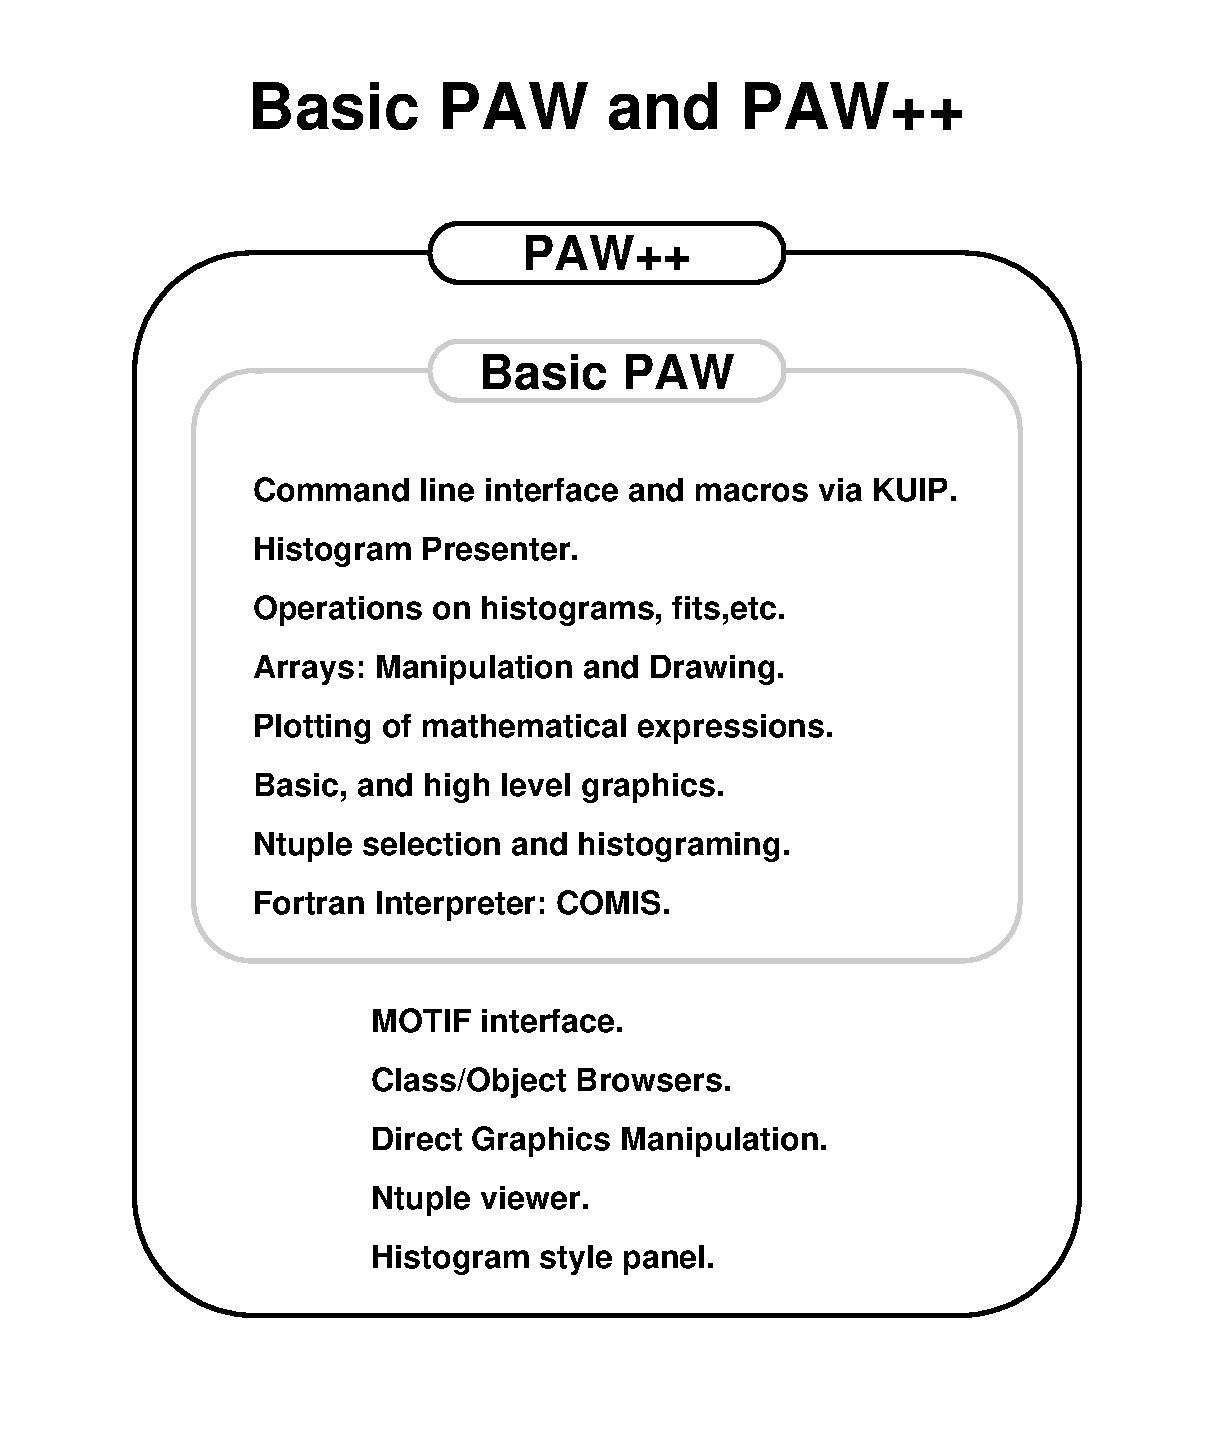
\includegraphics[width=.8\linewidth]{pawtut02.eps}
\caption{PAW and PAW++ compared}
\label{fig:paw++}
\end{figure}

At present \PAWPP{} is available on Unix workstations and VAX/VMS.

\PAWPP{} has, in addition to the conventional command line and macro types of
interface, the following dialogue modes:

\begin{DL}{Histogram style panel}
\item[Pull Down menus] They are useful to understand the command structure of
      the \XPAW{} system.
\item[Command panels] They give a ``panel representation'' of the commands.
\item[Object Browser] This is in many ways similar to the well-known browsers
      in the PC/MAC utilities or the visual tools on some workstations.
\item[Direct graphics] One can click in the graphics area and identify
      automatically which object has been selected. A pop-up menu appears
      with a list of possible actions on this object. For example, by clicking
      with the right mouse button on a histogram, one can make directly a
      gaussian fit, a smoothing etc.
      Pop-up menus are available by clicking on the \GW{} to
      automatically produce PostScript, Encapsulated PostScript, \LaTeX{} files
      or print the picture on your local printer.
\item[\HSP] Buttons are available to change
      histogram attributes, colours, line styles, fonts, and
      axes representation.
      2-D histograms can be rotated interactively. Zooming and rebinning can
      be performed interactively in real time.
\item[\NV] Just click on the Ntuple column name to histogram
      the column.
\end{DL}


The new system is largely self-explanatory. Only a subset of \XPAW{} has been
converted to this new user interface, but work is currently in progress to
offer many new facilities in future releases.

On all system on which \CERNLIB{} is installed, it is enough to type
\Ucom{paw++} to enter the system.

\PAWPP{} starts up with three windows on the screen:

\begin{DL}{The ``\PAWPP{} \EW''}
\item[The ``\PAWPP{} \EW'']
   includes a menu bar, a \TP, a current working directory indicator and an \IP.

\item[The ``\PAWPP{} Graphics 1'']
   window displays the graphics output from \HIGZ/\Xxi.
   Objects, e.g. histograms, displayed in the \GW{} can be
   manipulated by pointing at them, pressing the right mouse button and
   selecting an operation from the popup menu. Pointing at the edge of the
   \GW{} (between displayed object and window border) brings up a
   general popup menu. Up to 4 additional \GW{} can be opened by
   selecting ``Open New Window'' from this menu.

\item[The ``\PAWPP{} \MB'']
   displays all browsable classes and connected
   hbook files. Up to 4 additional browsers can be opened via the ``View'' menu
   of the ``\PAWPP{} \EW'' or via the ``Clone'' button on the
   browsers. For more information on the browsers see the ``Help'' menus.
\end{DL}


Figures~\ref{fig-pawppoverview1} on page \pageref{fig-pawppoverview1}
and \ref{fig-pawppoverview2} on page \pageref{fig-pawppoverview2} give
a detailed overview of the various windows of PAW++.

\begin{figure}[p]
\begin{center}
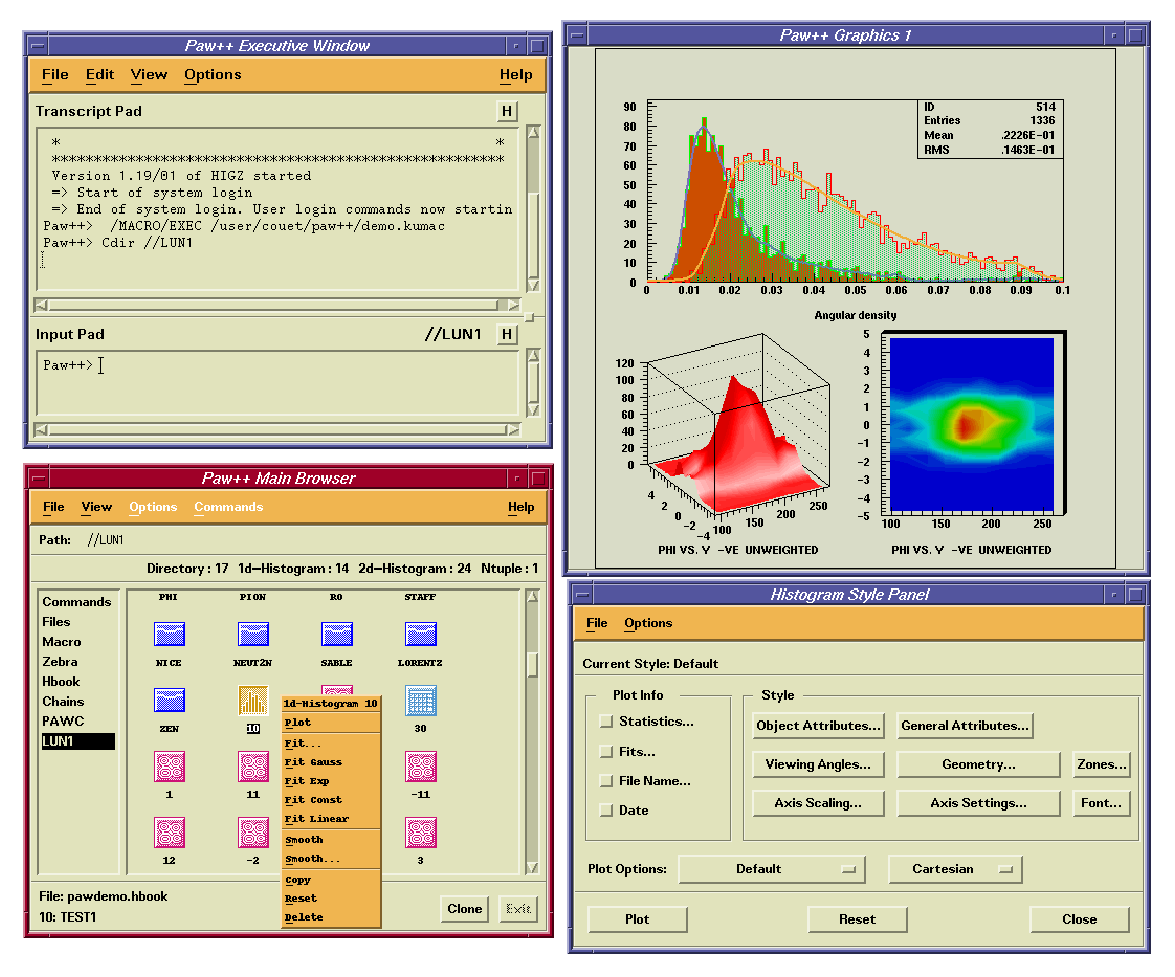
\includegraphics[width=\linewidth]{pawppoverview1.eps}
\end{center}
\small
\begin{UL}
\item The upper left corner is the \PAWPP{} \EW, with its \IP{}
      at the bottom and the \TP{} at the top.
\item The \PAWPP{} Browser, where the various entities (pictures, 1-D and
      2-D histograms and Ntuples) are all defined with their own symbol,
      is shown bottom left.  A ``pop-up'' menu has been activated for the 
      chosen 1-D histogram. Several actions like \texttt{Plot}, \texttt{Smooth},
      \texttt{Fit} etc... can be performed via this menu.
\item The \GW{} is seen top right. 
      A 1-D view of the data points and two 2-D views (a Surface-plot and a 
      colored contour plot) are shown.
      On the 1-D view, two 1-D histograms are 
      superimposed. The results of a ``smoothing'' type of fit to the data 
      points is also drawn. Information about the data and the fit can be found
      in the inserted window.
\item The \HSP{} at the lower right allows graphics
      attributes of the histogram to be controlled.
\end{UL}
\caption{PAW++ windows explained (I)}
\label{fig-pawppoverview1}
\end{figure}

\begin{figure}[p]
\begin{center}
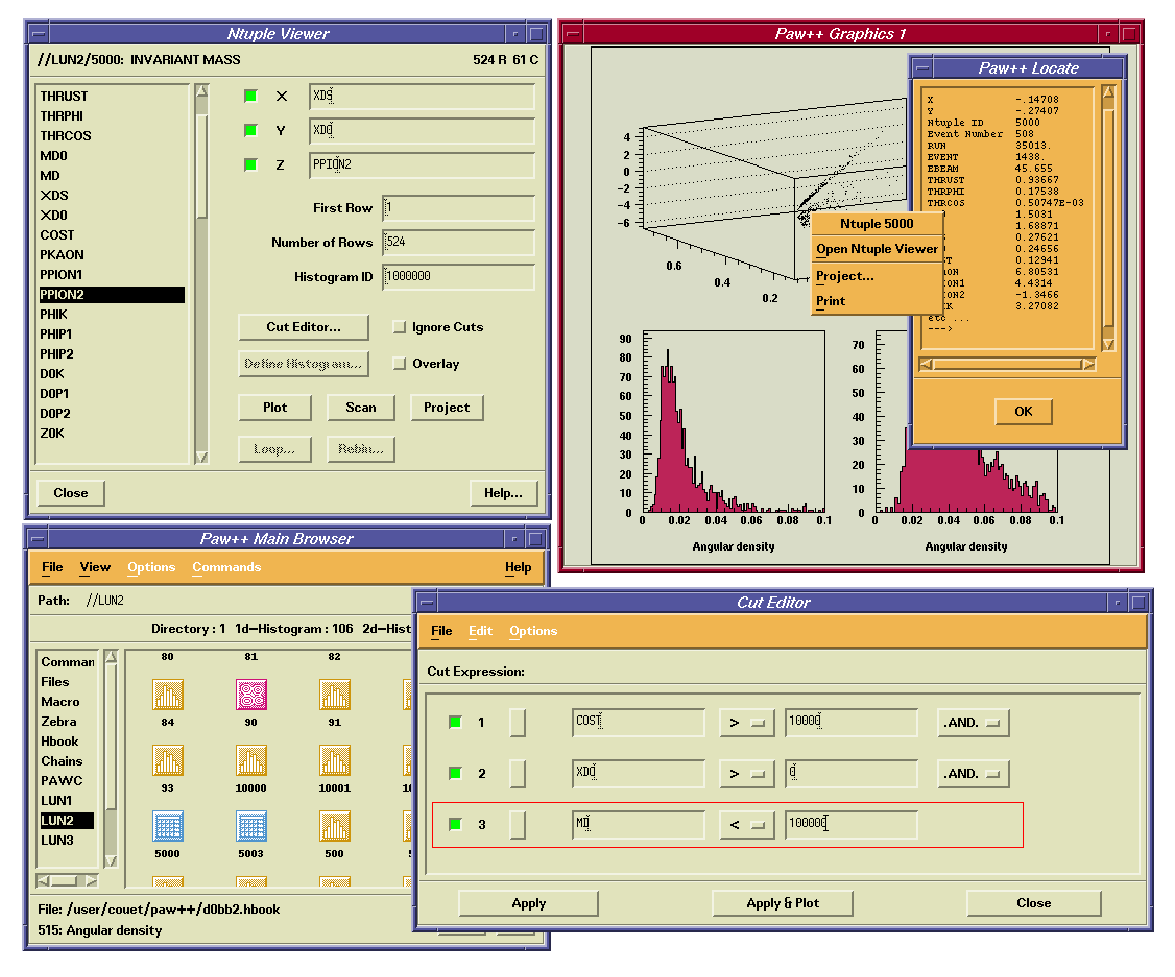
\includegraphics[width=\linewidth]{pawppoverview2.eps}
\end{center}
\small
\begin{UL}
\item The upper left corner shows the \NV.
      The left window shows the name of the various variables, characterizing
      the selected Ntuple. Other windows and press-buttons specify which
      combinations of the various variables and which events
      have to be treated (plotted, scanned, \ldots).
\item The lower left contains the \PAWPP{} Browser, with this time an Ntuple
      selected. A double on a Ntuple icon
      open automatically the \NV{} on the active Ntuple.
\item The \GW{} is seen top right and shows a 3-D view
      of the combination of three variables, whose cuts are
      specified with the \CE{} (see below).
\item Direct graphics interactions with Ntuple data are possible. Just
      by clicking on a point in the  \GW, the event description is displayed
      in the \PL{} window.
\item The \CE{} panel, shown at the lower right, allows
      various combinations of cuts to be specified and applied.
\end{UL}
\caption{PAW++ windows explained (II)}
\label{fig-pawppoverview2}
\end{figure}

\clearpage

\section{The Executive Window}

\PAWF[.7]{executive}

This window allows to type commands on the keyboard like in the normal \XPAW{}
system. In fact this window is the \Lit{kxterm} program provide with the \KUIP{}
package.

This terminal emulator combines the best features from the (now defunct) Apollo
DM pads (like: \IP{} and \TP, automatic file backup of \TP, string search in 
pads, etc.) and the Korn shell emacs-style command line editing and command line
recall mechanism.

Commands are typed in the \IP{} \NbDB{1} behind the application prompt. Via the
toggle buttons \Button{H} \NbDB{4} the \IP{} and/or \TP{} can be placed in hold
mode. In hold mode one can paste or type a number of commands into the \IP{} and
edit them without sending the commands to the application. Releasing the hold 
button will causes \Lit{kxterm} to submit all lines, upto the line containing 
the cursor, to the application. To submit the lines below the cursor, just move
the cursor down. In this way one can still edit the lines just before they are
being submitted to the application.


\begin{EnumZB}
\item In the \IP{} one can type, retrieve and edit command line with the help of
      a Korn shell emacs-style command line editing mode. See in appendix the 
      complete list of the editing keys.
\item The \TP{} \NbDB{2} shows the executed commands and command output.
      When in hold mode \NbDB{4} the transcript pad does not scroll to make 
      the new text
      visible. Mouse operations like ``Copy Paste'' are allowed in the 
      transcript pad. It is also possible to search a character string (see the
      menu bar description).
\item Every time the current directory is changed, the {\bf Current working 
      directory indicator} is updated. The current working directory can be 
      changed by clicking on a item in the {\bf PATH window} of the \MB{} or
      by clicking on a icon directory in the \MB{} itself.
\item Hold buttons.
\end{EnumZB}
\begin{EnumZW}
\item Allows manipulation of the \TP. 
\item Allows character string seach, copy/paste in the \TP.
\item Allows to invoke other panel. 
\item Some general settings are available in this menu. 
\item Online help.
\end{EnumZW}


\subsection{The \EW{} menu bar}
In this section, is describe the full functionality of the pull down
menu available in the Menu Bar of the \EW.

\PAWFR{menu1}

\subsubsection{File}

\begin{PAWf}{file1}
\begin{DLsf}{Save Transcript As ...}
\item[About Kxterm...]
         Displays version information about Kxterm.
\item[About \lab Application\rab...]
         Displays version information about the application
         Kxterm is servicing.
\item[Save Transcript]
         Write the contents of the transcript pad to the current
         file. If there is no current file a file selection box
         will appear.
\item[Save Transcript As...]
         Write the contents of the transcript pad to a user-specified
         file.
\item[Print...]
         Print the contents of the transcript pad (not yet implemented).
\item[Kill]
         Send a SIGINT signal to the application to cause it to
         core dump. This is useful when the application is hanging or
         blocked. Use only in emergency situations.
\item[Exit]
         Exit Kxterm and the application. When this option is selected
         or when \Lit{EXIT} is typed in the \IP, the following panel is 
         displayed:
\end{DLsf}
\end{PAWf}

\begin{PAWf}[.4]{exit}
\begin{EnumZB}
\item  The exit is performed.
\item  The exit procedure is canceled.
\end{EnumZB}
\end{PAWf}

\subsubsection{Edit}
\begin{PAWf}{edit1}
\begin{DLsf}{Search ...}
\item[Cut]
         Remove the selected text. The selected text is written to the
         Cut and Paste buffer. Using the ``Paste'' function, it can be
         written to any \Xxi program. In the transcript pad ``Cut''
         defaults to the ``Copy'' function.
\item[Copy]
         Copy the selected text. The selected text is written to the
         Cut and Paste buffer. Using the ``Paste'' function, it can be
         written to any \Xxi program.
\item[Paste]
         Insert text from the Cut and Paste buffer at the cursor location
         into the \IP.
\item[Search...]
         Search for a text string in the transcript pad.
\end{DLsf}
\end{PAWf}

\subsubsection{View}

\begin{PAWf}{view}
\begin{DLsf}{Command Panel}
\item[Show Input]
         Show in a window all commands entered via the \IP.
\item[Command Panel]
\item[Browser]
\item[Style Panel]
\end{DLsf}
\end{PAWf}

\subsubsection{Options}

\begin{PAWf}{option1}
\begin{DLsf}{Clear Transcript Pad}
\item[Clear Transcript Pad]
         Clear all text off of the top of the transcript pad.
\item[Echo Command]
         Echo executed commands in transcript pad.
\item[Timing]
         Report command execution time (real and CPU time).
\item[Iconify]
         Iconify Kxterm and all windows of the application.

\end{DLsf}
\end{PAWf}

\subsubsection{Help}
\begin{DLsf}{On Edit Keys}
\item[On Kxterm]
         The help you are currently reading.
\item[On Edit Keys]
         Help on the emacs-style edit key sequences.
\end{DLsf}

\section{The Main Browser}

The \KUIP/\MOTIF{} Browser interface is a general tool to display and
manipulate a tree structure of objects which are defined either by \KUIP{}
itself (commands, files, macros, etc.) or by the application.

The ``Clone'' button at the bottom creates a new independent browser window.
The ``Exit'' button destroys the browser window. The \MB{} cannot be
destroyed (only iconized).

The middle part of the browser is divided into two windows:

\begin{enumerate}
\item The left hand ``class window'' shows the list of all currently connected
   classes of objects.  Some classes, e.g. the command tree and the file
   system, are predefined.  Other classes allow to attach new files using the
   commands in the ``File'' menu.  Clicking with the left mouse button on
   one of
   the items in the class window displays its content in the other window.
   Pressing the right mouse button inside the class window shows a popup menu
   of possible operations, e.g. creating a new object in the current
   directory.

\item The right hand ``object window'' shows the content of the currently
   selected class directory.  The ``View'' menu allows the change the way
   objects are displayed, i.e. to choose the icon size and the amount of
   information shown for each object.  Objects are selected by clicking on
   them with the left mouse button.  Pressing the right mouse button pops up a
   menu of possible operations depending on the object type.
\end{enumerate}

   An item in a popup menu is selected by pointing at the corresponding line
   and releasing the right mouse button.  Double clicking with the left mouse
   button is equivalent to selecting the first menu item.

   Each menu item executes a command sequence where the name of the selected
   object is filled into the appropriate place.  By default the command is
   executed immediately whenever possible. The commands executed can be seen
   by selecting ``Echo Commands'' in the ``Options'' menu of the \EW.
   In case some mandatory parameters are missing a panel is displayed
   where the remaining arguments have to be filled in.  The command is
   executed then by pressing the ``OK'' or ``Execute'' button in that panel.
   (If it is not the last one in the sequence of commands bound to the menu item
   the application is blocked until the ``OK'' or ``Cancel'' button is pressed.)

   The immediate command execution can be inhibited by holding down the
   CTRL-key BEFORE pressing the right mouse button.  Some popup menus also
   contain different menu item for immediate and delayed execution, e.g.
   ``Execute'' and ``Execute...'' for class ``Commands''

   The path of the currently selected directory is always displayed below the
   menu bar.  The directory can be changed by pointing at the tail of the
   wanted subpath and clicking the left mouse button.  Clicking a second time
   on the same path segment performs the directory change and updates the
   object window.  To go downwards in the directory hierarchy double click on
   the subdirectory displayed in the object window.

\PAWF[.8]{browser}

\begin{minipage}[t]{.65\linewidth}
\begin{EnumZB}
\item Current PATH (``PATH window'').
\item Class window.
\item Name of file currently selected in the class window.
\item Name of the object currently selected in the object window.
\item Number and type of object currenlty in the the object window.
\item Object window.
\end{EnumZB}
\end{minipage}\hfill
\begin{minipage}[t]{.31\linewidth}
\begin{EnumZW}
\item File menu.
\item View menu.
\item Options menu.
\item Commands menu.
\item Help menu.
\item Clone button.
\item Exit button.
\end{EnumZW}
\end{minipage}

\subsection{The objects in the ``object window''}
This section describes all the \PAWPP{} object available in the \MB{}.

\subsubsection{\HBOOK{} files}
\begin{ICON}{hbookicon}
Double click with the left mouse button on this icon, open the corresponfing
\HBOOK{} file with the command \Lit{HISTOGRAM/FILE}.
\end{ICON}

Select a {\bf \HBOOK{} files} icon with the left mouse button and press
the right mouse button to obtain the following menu:

\begin{PAWf}{hbookmenu}
\begin{DLsf}{Open Update Mode}
\item[Open]              Open the highlighted \HBOOK{} file in read-only mode.
\item[Open Update Mode]  Open the highlighted \HBOOK{} file in update mode.
\end{DLsf}
\end{PAWf}

Note that the \HBOOK{} file name is displayed in the menu title.


\subsubsection{1D histograms}
\begin{ICON}{1dicon}
Double click with the left mouse button on this icon, produce the plot of the
corresponding histogram with the command  \Lit{HISTOGRAM/PLOT}. The histogram
becomes the current histogram for the \HSP.
\end{ICON}

Select a {\bf 1D histograms} icon with the left mouse button and press
the right mouse button to obtain the following menu:

\begin{PAWf}[.25]{1dmenu}
\begin{DLsf}{Fit Linear}
\item[Plot]         Plot the corresponding histogram (default action). The
                    histogram becomes the current histogram for the 
                    {\bf Histogram Style Panel}.
\item[Fit...]       Perform the command \Lit{Histo/Fit} on the corresponding
                    histogram. The command panel is automatically displayed
\item[Fit Gauss]    Perfom a gaussian fit on the corresponding histogram.
\item[Fit Exp]      Perform an exponential fit on the corresponding histogram.
\item[Fit Const]    Perform a \Lit{P0} fit on the corresponding histogram.
\item[Fit Linear]   Perform a \Lit{P1} fit on the corresponding histogram.
\item[Smooth]       Smooth the corresponding histogram.
\item[Smooth...]    Perform the command \Lit{Smooth} on the corresponding
                    histogram. The command panel is automatically invoked.
\item[Copy ]        Copy corresponding histogram onto an other histogram.
                    The command panel is automatically invoked.
\item[Reset ]       Reset the corresponding histogram.
\item[Delete]       Delete the corresponding histogram.
\end{DLsf}
\end{PAWf}

Note that the histogram identifier is displayed in the menu title.


\subsubsection{2D histograms}
\begin{ICON}{2dicon}
Double click with the left mouse button on this icon, produce the plot of the
corresponding histogram with the command  \Lit{HISTOGRAM/PLOT}. The histogram
becomes the current histogram for the \HSP.
\end{ICON}

Select a {\bf 2D histograms} icon with the left mouse button and press
the right mouse button to obtain the following menu:

\begin{PAWf}[.25]{2dmenu}
\begin{DLsf}{Project X}
\item[Plot]         Plot the corresponding histogram (default action). The
                    histogram becomes the current histogram for the \HSP.
\item[Project X]    Generate the \Lit{X} projection, perform the projection
                    and plot the result (commands \Lit{ProX}, \Lit{Hi/Proj},
                    and \Lit{Hi/Plot}).
\item[Project Y]    Generate the \Lit{Y} projection, perform the projection
                    and plot the result (commands \Lit{ProY}, \Lit{Hi/Proj},
                    and \Lit{Hi/Plot}).
\item[Slice X]      Generate the \Lit{X} slices, perform the projection
                    and plot the first slice (commands \Lit{SliX},
                    \Lit{Hi/Proj}, and \Lit{Hi/Plot}).
\item[Slice Y]      Generate the \Lit{Y} slices, perform the projection
                    and plot the first slice (commands \Lit{SliY},
                    \Lit{Hi/Proj}, and \Lit{Hi/Plot}).
\item[Band X]       Generate the \Lit{X} bands, perform the projection
                    and plot the first band (commands \Lit{BanX},
                    \Lit{Hi/Proj}, and \Lit{Hi/Plot}).
\item[Band Y]       Generate the \Lit{Y} bands, perform the projection
                    and plot the first band (commands \Lit{BanY},
                    \Lit{Hi/Proj}, and \Lit{Hi/Plot}).
\item[Smooth]       Smooth the corresponding histogram.
\item[Smooth...]    Perform the command \Lit{Smooth} on the corresponding
                    histogram. The command panel is automatically invoked.
\item[Copy ]        Copy corresponding histogram onto an other histogram.
                    The command panel is automatically invoked.
\item[Reset ]       Reset the corresponding histogram.
\item[Delete]       Delete the corresponding histogram.
\end{DLsf}
\end{PAWf}

Note that the histogram identifier is displayed in the menu title.

\subsubsection{Ntuples}
\begin{ICON}{nticon}
Double click with the left mouse button on this icon, open the \NV{} on the
corresponding Ntuple.
\end{ICON}

Select a {\bf Ntuples} icon with the left mouse button and press
the right mouse button to obtain the following menu:

\begin{PAWf}{ntmenu}
\begin{DLsf}{[Open Ntuple Viewer}
\item[Open Ntuple Viewer]    Open Ntuple Viewer on the highlighted Ntuple.
\item[Project...]            Project the highlighted Ntuple. The Command
                             panel \Lit{Ntuple/Proj} is automatically invoked.
\item[Print]                 Print the highlighted Ntuple (Command
                             \Lit{Ntuple/Print)}.
\end{DLsf}
\end{PAWf}

Note that the Ntuple identifier is displayed in the menu title.


\subsubsection{\XPAW{} commands}
\begin{ICON}{cmdicon}
Double click with the left mouse button on this icon, execute the corresponding
\XPAW{} command.
\end{ICON}

Select a {\bf \XPAW{} commands} icon with the left mouse button and press
the right mouse button to obtain the following menu:

\begin{PAWf}[.2]{cmdmenu}
\begin{DLsf}{Set Command}
\item[Execute]      Execute the command with the default parameters. If
                    a mandatory parameter is missing, the command panel
                    is automatically invoked.
\item[Execute...]   Display the command panel.
\item[Help]         Display the help on the command.
\item[Usage]        Display the command usge in the \TP{} of the \EW.
\item[Manual]       Equivalent to \Lit{HELP}.
\item[Set Command]  This command becomes the one executed when a directive
                    typed on the keyboard is not an existing \XPAW{} command.
\item[Deactivate]   The command is deactivated.
\end{DLsf}
\end{PAWf}

Note that the command name is displayed in the menu title.


\subsubsection{Deactivated \XPAW{} commands}
\begin{ICON}{dcmdicon}
Double click with the left mouse button on this icon, execute the help on
corresponding \XPAW{} command.
\end{ICON}

Select a {\bf Deactivated \XPAW{} commands} icon with the left mouse button
and press the right mouse button to obtain the following menu:

\begin{PAWf}{dcmdmenu}
\begin{DLsf}{Activate}
\item[Help]         Display the help on the command.
\item[Activate]     The command is activated.
\end{DLsf}
\end{PAWf}

Note that the deactivated command name is displayed in the menu title.

\subsubsection{Up}
\begin{ICON}{upicon}
Double click with the left mouse button on this icon, allow to go one level up
in the directory tree. This icon is alway the first one of the {\bf content
window}.
\end{ICON}

Select a {\bf Up} icon with the left mouse button and press
the right mouse button to obtain the following menu:

\begin{PAWf}{upmenu}
\begin{DLsf}{List}
\item[List]         Allow to go one level up in the directory tree.
\end{DLsf}
\end{PAWf}

\subsubsection{Directory}
\begin{ICON}{diricon}
Double click with the left mouse button on this icon, change the current
working directory.
\end{ICON}

Select a {\bf Directory} icon with the left mouse button and press
the right mouse button to obtain the following menu:

\begin{PAWf}{dirmenu}
\begin{DLsf}{List}
\item[List] Change the current working directory.
\end{DLsf}
\end{PAWf}

\subsubsection{PostScript files}
\begin{ICON}{psicon}
Double click with the left mouse button on this icon, invoke the ghostview
on the corresponding file.
\end{ICON}

Select a {\bf PostScript files} icon with the left mouse button and press
the right mouse button to obtain the following menu:

\begin{PAWf}{psmenu}
\begin{DLsf}{Delete}
\item[View]         Invoke GhostView on the file.
\item[Edit]         Edit the file.
\item[Print]        Print the file.
\item[Delete]       Delete the file.
\end{DLsf}
\end{PAWf}

\subsubsection{Read-Write files}
\begin{ICON}{rwicon}
Double click with the left mouse button on this icon, invoke the editor on the
corresponding file.
\end{ICON}

Select a {\bf Read-Write files} icon with the left mouse button and press
the right mouse button to obtain the following menu:

\begin{PAWf}{rwmenu}
\begin{DLsf}{Delete}
\item[Edit]         Edit the file.
\item[View]         Read the file.
\item[Delete]       Delete the file.
\end{DLsf}
\end{PAWf}

Note that the file name is displayed in the menu title.


\subsubsection{Read-only files}
\begin{ICON}{roicon}
Double click with the left mouse button on this icon, invoke the editor in view
mode on the corresponding file.
\end{ICON}

Select a {\bf Read-only files} icon with the left mouse button and press
the right mouse button to obtain the following menu:

\begin{PAWf}{romenu}

\begin{DLsf}{Delete}
\item[View]         Read the file.
\item[Delete]       Delete the file.
\end{DLsf}
\end{PAWf}

Note that the file name is displayed in the menu title.


\subsubsection{No-access files}
\begin{ICON}{naicon}
Double click with the left mouse button on this icon, invoke the shell command
\Lit{chmod} on the corresponding file.
\end{ICON}

Select a {\bf No-access files} icon with the left mouse button and press
the right mouse button to obtain the following menu:

\begin{PAWf}{namenu}
\begin{DLsf}{Chmod}
\item[Chmod]         Try to change the permissions of the file.
\end{DLsf}
\end{PAWf}

Note that the file name is displayed in the menu title.


\subsubsection{Executable files}
\begin{ICON}{xicon}
Double click with the left mouse button on this icon, invoke the command
\Lit{SHELL} on the corresponding file.
\end{ICON}

Select a {\bf Executable files} icon with the left mouse button and press
the right mouse button to obtain the following menu:

\begin{PAWf}{xmenu}
\begin{DLsf}{Delete}
\item[Execute]         Invoke the command \Lit{SHELL} on the file.
\item[Execute...]      Open the command panel \Lit{SHELL} with the file name.
\item[Edit]            Edit the file.
\item[View]            Read the file.
\item[Delete]          Delete the file.
\end{DLsf}
\end{PAWf}

Note that the file name is displayed in the menu title.


\subsubsection{\XPAW{} Macros}
\begin{ICON}{macroicon}
Double click with the left mouse button on this icon, execute the
corresponding macro.
\end{ICON}

Select a {\bf \XPAW{} Macros} icon with the left mouse button and press
the right mouse button to obtain the following menu:

\begin{PAWf}{macromenu}
\begin{DLsf}{Delete}
\item[Exec]            Execute the macro.
\item[Exec...]         Open the command panel \Lit{EXEC} with the macro name.
                       It is useful to give parameters to the macro.
\item[Edit]            Edit the macro.
\item[View]            Read the macro.
\item[Delete]          Delete the macro.
\end{DLsf}
\end{PAWf}

Note that the macro name is displayed in the menu title.

\subsubsection{Pictures}
\begin{ICON}{picticon}
Double click with the left mouse button on this icon, plot the corresponding
picture.
\end{ICON}

Select a {\bf Pictures} icon with the left mouse button and press
the right mouse button to obtain the following menu:

\begin{PAWf}[.25]{pictmenu}
\begin{DLsf}{Do PostScript}
\item[Plot]             Plot the highlighted picture.
\item[Do PostScript]    Produce the \PS{} file \Lit{PNAME.ps}, where
                        \Lit{PNAME} is the name of the highlighted picture.
\item[Create]           Create a new picture. The command panel
                        \Lit{Picture/Create} is automatically invoked.
\item[Rename]           Rename the highlighted picture. The command panel
                        \Lit{Picture/Rename} is automatically invoked.
\item[Delete]           Rename the highlighted picture.
\end{DLsf}
\end{PAWf}

\subsubsection{Chains}
\begin{ICON}{chainicon}
Double click with the left mouse button on this icon, allow to go one level
deeper in the chain tree.
\end{ICON}

Select a {\bf Chains} icon with the left mouse button and press
the right mouse button to obtain the following menu:

\begin{PAWf}[.2]{chainmenu}
\begin{DLsf}{Delete Chain}
\item[List]                      List the available chains.
\item[Show Tree]                 Show the tree from the highlighted chain.
\item[Delete Chain]              Delete the highlighted chain.
\end{DLsf}
\end{PAWf}

\subsubsection{Last chain level}
\begin{ICON}{chainlicon}
Last chain element.
\end{ICON}

Select a {\bf Last chain level} icon with the left mouse button and press
the right mouse button to obtain the following menu:

\begin{PAWf}[.2]{chainlmenu}
\begin{DLsf}{Delete Chain Entry}
\item[List]                      List the available chains.
\item[Delete Chain Entry]        Delete the highlighted chain element.
\end{DLsf}
\end{PAWf}

\subsubsection{\ZEBRA{} Stores}
\begin{ICON}{storeicon}
Double click with the left mouse button on this icon, allow to go inside the
corresponding \ZEBRA{} store.
\end{ICON}

Select a {\bf \ZEBRA{} Stores} icon with the left mouse button and press
the right mouse button to obtain the following menu:

\begin{PAWf}{storemenu}
\begin{DLsf}{Show store DZSTOR}
\item[List]                      Display divisions of the store 
\item[Show store DZSTOR] Show parameters of the store (\texttt{CALL
                         DZSTOR})
\end{DLsf}
\end{PAWf}

\subsubsection{\ZEBRA{} Divisions}
\begin{ICON}{divicon}
Double click with the left mouse button on this icon, allow to go inside the
corresponding \ZEBRA{} division.
\end{ICON}

Select a {\bf \ZEBRA{} Divisions} icon with the left mouse button and press
the right mouse button to obtain the following menu:

\begin{PAWf}{divmenu}
\begin{DLsf}{Set filter for banks}
\item[List]                      Display banks of the division as icons.
\item[Display division]          Show layout of banks in divisions graphically.
\item[Snap division]             Show a snapshot of division parameters.
                                 (\texttt{CALL DZSNAP}).
\item[Verify division]           Verify division (\texttt{CALL DZVERI}).
\item[Collect garbage]           \texttt{CALL MZGARB} in selected division.
\item[Set filter for banks]      Allow to display only banks whose hollerith.
                                 identifiers  match a wild card selection.
\end{DLsf}
\end{PAWf}

\subsubsection{\ZEBRA{} Banks}
\begin{ICON}{bankicon}
Double click with the left mouse button on this icon, draw the bank tree from
the corresponding \ZEBRA{} bank.
\end{ICON}

Select a {\bf \ZEBRA{} Banks} icon with the left mouse button and press
the right mouse button to obtain the following menu:

\begin{PAWf}{bankmenu}
\begin{DLsf}{Show cont documented}
\item[Display bank tree]         Display graphically the structure below the 
                                 selected bank (see picture banktree.eps).
\item[Show cont documented]      Display the data of the bank with their
                                 description if a documentation data base is
                                 provided (see CERN Q101).
\item[DZ Show contents]          \texttt{CALL DZSHOW} fore selected bank.
\item[Show system words]         List contents of the links and system words.
\item[Survey bank tree]          \texttt{CALL DZSURV} for selected bank.
\item[Put into vector]           Put data contents of the bank into a KUIP
                                 vector.
\item[Show documentation]        Display the documentation for the bank 
                                 (if provided).
\item[Edit documentation]        Edit a bank descriptor, if no available yet
                                 provide a template.
\item[Modify data words]         Self explaining.
\item[Drop bank (tree)]          Self explaining.
\end{DLsf}
\end{PAWf}

\subsubsection{\RZ{} Files}
\begin{ICON}{rzicon}
Double click with the left mouse button on this icon, allow to go inside the
corresponding \ZEBRA/\RZ{} file.
\end{ICON}

Select a {\bf \RZ{} Files} icon with the left mouse button and press
the right mouse button to obtain the following menu:

\begin{PAWf}{rzmenu}
\begin{DLsf}{Show key definition}
\item[Close RZfile]        Self explaining.
\item[List]                Display keys.
\item[List directory]      \texttt{CALL RZLDIR}.
\item[Show key definition] self explaining.
\item[Set filter on keys]  Allow to display only entries whose key words
                           match a wild card selection.
\item[Show status]         \texttt{CALL RZSTAT}.
\end{DLsf}
\end{PAWf}

\subsubsection{\RZ{} Directories}
\begin{ICON}{rzdiricon}
Double click with the left mouse button on this icon, allow to go inside the
corresponding \ZEBRA/\RZ{} directory.
\end{ICON}

Select a {\bf \RZ{} Directories} icon with the left mouse button and press
the right mouse button to obtain the following menu:

\begin{PAWf}[.25]{rzdirmenu}
\begin{DLsf}{List directory (RZLDIR)}
\item[List]                      List the highlighted \RZ{} directory.
\item[List directory (RZLDIR)]   Perform \Rind{RZLDIR} on the
                                 highlighted \RZ{} directory.
\item[Show key definition]       Display the key definition.
\item[Set filter on keys]        Defines a filter on the keys.
\end{DLsf}
\end{PAWf}

\subsubsection{\RZ{} Keys}
\begin{ICON}{keyicon}
Double click with the left mouse button on this icon, allow to read into memory
the corresponding \ZEBRA/\RZ{} key.
\end{ICON}

Select a {\bf \RZ{} Keys} icon with the left mouse button and press
the right mouse button to obtain the following menu:

\begin{PAWf}{keymenu}
\begin{DLsf}{Read key into memory}
\item[Read key into memory] Allow to inspect the data of a key.
\item[Show key definition]  Self explaining.
\item[Show key words]       Self explaining.
\item[Set filter on keys]   See above.
\end{DLsf}
\end{PAWf}

\subsection{The \MB{} Menu Bar}
In this section, is describe the full functionality of the pull down
menu available in the Menu Bar of the \MB.

\PAWF{browsermenubar}

\subsubsection{File}

\begin{PAWf}[.25]{browsermenubarfile}
\begin{DLsf}{Close Hbook file}
\item[Open Hbook file]      Display the {\bf Open Arguments} panel (see after).
\item[Close Hbook file]     Display the {\bf Close Arguments} panel (see after).
\end{DLsf}
\end{PAWf}

\newpage

\PAWF[.7]{openhbook}

\begin{EnumZW}
\item Toggle buttons to choose the openning mode.
\item Filter apply on the file list \NbDB{6}.
\item Possible logical units. Only the free units are displayed.
      The next free unit is highlighted. Any other unit is invalid. 
\item Possible record length. A record length of \Lit{0} means that the
      system will compute the correct one automatically.
\end{EnumZW}
\begin{EnumZB}
\item The file is open and this panel is closed.
\item File name of the opened file.
\item Apply the filter defined in \NbDW{2}.
\item List of the subdirectories available. Double click
      on a directory name change the current directory.
\item Cancel the current opened panel and clode it.
\item List of the file in the current directory matching
      the filter.
\item Help
\end{EnumZB}
Note that a double click with the left mouse button on a
\HBOOK{} file icon in the object window of the \MB{} open also 
the \HBOOK{} file.
This panel is usefull to specify a filter different form
the default filter \Lit{*.hbook} used in the object window.

\begin{PAWf}[.55]{closehbook}
\begin{EnumZW}
\item List of the currently connected hbook files.
\item A simple click with the left mouse button a file name
      in the connected files list, highlight the filename
      and put it in the {\bf Close file} field \NbDW{3}.
\item Name of the file to be closed. This field can be filled
      directly by tipyng on the keyboard, or by a simple click
      with the left mouse button in the {\bf Connected Files}
      list \NbDW{1}.
\end{EnumZW}
\begin{EnumZB}
\item When a file is selected, clicking on this button or
      typing \Lit{<CR>} allows to perform the action (close
      the file) and close the panel.
\item Close the selcted file and leave the panel opened.
\item Cancel the current operation and close the panel.
\item  Give some help.
\end{EnumZB}
\end{PAWf}

\subsubsection{View}

This pull down menu allows to define the ``viewing'' for the objects
in the ``object window'' of the \MB.

\begin{PAWf}[.2]{browsermenubarview}
\begin{DLsf}{Small Icons}
\item[Icons]       The objects are represented with big icons (default).
\item[Small Icons] The objects are represented with small icons.
\item[No Icons]    Only the object identifier and type are displayed.
\item[Titles]      Small icons, objects identifiers and titles are displayed.
\item[Select All]  All the objects are selected.
\item[Filter...]   Apply a filter on object names.
\end{DLsf}
\end{PAWf}

\begin{PAWf}[.6]{viewicon}
Icons: icons and the object identifiers are displayed.
\end{PAWf}

\begin{PAWf}[.6]{viewsmallicon}
Small Icons: small icons  and the object identifiers are displayed.
\end{PAWf}

\begin{PAWf}[.6]{viewnoicon}
No Icons : object identifiers and titles are displayed.
\end{PAWf}

\begin{PAWf}[.6]{viewtitle}
Titles : small icons  and the object identifiers and titles are displayed.
\end{PAWf}

\subsubsection{Options}

\begin{PAWf}{browsermenubaroptions}
\begin{DLsf}{Command Panel Help...}
\item[Raise Window]                    Raise a given window.
\item[Command Argument Panel...]       Get help on a given command.
\end{DLsf}
\end{PAWf}

\subsubsection{Commands}

This menu allows to access the tree of the \XPAW{} commands. Only the
top levels are describe in this section. Note the tree of the \XPAW{}
commands can also be accessed via the item ``Commands'' in the ``PATH Window''
of the \MB.

\begin{PAWf}[.15]{browsermenubarcommands}
\begin{DLsf}{Histogram}
\item[Kuip]         Command Processor commands.
\item[Macro]        Macro Processor commands.
\item[Vector]       Vector Processor commands.
\item[Histogram]    Manipulation of histograms, Ntuples.
\item[Function]     Operations with Functions. Creation and plotting.
\item[Ntuple]       Ntuple creation and related operations.
\item[Graphics]     Interface to the graphics packages HPLOT and HIGZ.
\item[Picture]      Creation and manipulation of HIGZ pictures.
\item[Fortran]      Interface to MINUIT, COMIS, SIGMA and FORTRAN Input/Output.
\item[Network]      To access files on remote computers.
\item[Dzdoc]        Access Dzdoc
\end{DLsf}
\end{PAWf}

\subsubsection{Help}

\subsection{Information Windows}

\subsubsection{Top}

\PAWF[.6]{browserinfotop}

On the top of the \MB{} is displayed the current directory PATH and
the content of the current directory i.e. the number of objects of each
type.

\subsubsection{Bottom}

\PAWF[.6]{browserinfobottom}

On the bottom of the \MB{} is displayed the name of the current
file (\HBOOK{} files for example) in which the objects are stored.
If the objects are not stored in a file (like the commands), the
file name is just blank. Below the file name, the full name of the
currently selected object is displayed.

\newpage

\subsection{Content Window}

In this section are describe the different menu available in the 
``Content Window''.

\subsubsection{Commands}

\begin{PAWf}[.55]{contentcommands}
\begin{DLsf}{Set Default}
\item[List]         List the content of the current menu.
\item[Set Default]  Set the root for searching commands to /.
\item[Help]         Display some help.
\end{DLsf}
\end{PAWf}

\subsubsection{Files}
\begin{PAWf}[.55]{contentfiles}
\begin{DLsf}{Chdir to ...}
\item[List]          List the content of the current working directory (OS).
\item[Chdir to ...]  Change directory.
\item[Edit]          Edit a file.
\item[Help]          Display some help.
\end{DLsf}
\end{PAWf}

\subsubsection{Macro}
\begin{PAWf}[.55]{contentmacro}
\begin{DLsf}{Help}
\item[List] List all the macros in the current working directory.
\item[Edit] Edit a macro.
\item[Help] Display some help.
\end{DLsf}
\end{PAWf}

\subsubsection{Zebra}

\begin{PAWf}[.55]{contentzebra}
\begin{DLsf}{Open bank doc Rzfile}
\item[List]                  List the \ZEBRA{} file connected.
\item[Open bank doc Rzfile]  Open bank doc Rzfile.
\item[Add doc directory]     Add doc directory.
\item[Put doc into Rzfile]   Put doc into Rzfile.
\item[Display bank tree]     Display bank tree.
\item[Help]                  Display some help.
\end{DLsf}
\end{PAWf}

\subsubsection{Hbook}
\begin{PAWf}[.55]{contenthbook}
\begin{DLsf}{Help}
\item[List]  List all the \HBOOK{} files in the current working directory.
\item[Help]  Display some help.
\end{DLsf}
\end{PAWf}

\subsubsection{Chains}

\begin{PAWf}[.55]{contentchain}
\begin{DLsf}{Delete All Chains}
\item[List]               List the chains currently in memory.
\item[Delete All Chains]  Delete all the chains from memory.
\item[Help]               Display some help.
\end{DLsf}
\end{PAWf}

\begin{PAWf}[.4]{chaintree}
This panel allows to navigate in the chain tree. Just clicking on a
chain name change the level from which the chain will be traversed.
\end{PAWf}

\subsubsection{PAWC}

\begin{PAWf}[.4]{contentpawc}
\begin{DLsf}{Create N-tuple}
\item[List]           List all the \HBOOK{} objects in memory.
\item[Create 1d]      Create a 1d histogram.
\item[Create Profile] Create a Profile histogram.
\item[Create Var-Bin] Create a variable bin size histogram.
\item[Create 2d]      Create a 2d histogram.
\item[Create N-tuple] Create a row wise Ntuple histogram.
\item[Clear]          Delete histograms from memory.
\item[Help]           Provide some help.
\end{DLsf}
\end{PAWf}

\subsubsection{Hbook Files (//LUNn)}

\begin{PAWf}[.4]{contentlun}
\begin{DLsf}{Write from //PAWC...}
\item[List]                 List all the \HBOOK{} objects in this file.
\item[Copy to //PAWC]       Copy the highlighted \HBOOK{} object in memory.
\item[Add to //PAWC]        Add the highlighted \HBOOK{} object in memory.
\item[Write from //PAWC...] Save the highlighted \HBOOK{} object on disk.
\item[Create N-tuple]       Create a row wise Ntuple histogram.
\item[Clear]                Delete histograms from disk.
\item[Close]                Close the selected hbook file
\item[Help]                 Provide some help.
\end{DLsf}
\end{PAWf}

\section{Graphics}

\begin{PAWf}[.6]{graphics}
\PAWPP{} allows direct graphics manipulation of the objects like Histograms
or Ntuples. To perform actions on object from the \GW, it is
enough to move the mouse cursor on the \GW{} and to click with the
right mouse button on the object. A pull down menu will be displayed according
to the object picked. In this section are described the different menus
available in the \GW.
\end{PAWf}

\subsection{The \GW}
When no object is picked in the \GW{} for instance when the
background of the window is picked the following menu is displayed.

\begin{PAWf}[.28]{graphicswindow}
\begin{DLsf}{Do Encapsulated PostScript...}
\item[Plot]                           PLot the current picture.
\item[Style Panel...]                 Invoke the \HSP.
\item[Double Buffer On]               Set the double buffer on.
\item[Double Buffer Off]              Set the double buffer off.
\item[Do PostScript...]               Generate the Postscipt file \Lit{paw.ps}.
\item[Do Encapsulated PostScript...]  Generate the Encapsulated Postscipt file
                                      \Lit{paw.eps}.
\item[Do LaTex...]                    Generate the LaTex file \Lit{paw.tex}.
\item[Print]                          Print the current picture.
\item[Open New Window]                Open a new window.
\item[Close Window]                   Close the current window.
\item[Activate Window]                Activate the current window.
\item[Deactivate Window]              Deactivate the current window.
\end{DLsf}
\end{PAWf}

\newpage

\subsection{Ntuple}
An Ntuple picked in \GW{} with the right mouse button displays
the following menu:

\begin{PAWf}[.23]{graphicsntuple}
\begin{DLsf}{Open Ntuple Viewer}
\item[Open Ntuple Viewer]     Open the Ntuple browser.
\item[Project...]             Project the picked ntuple.
\item[Print]                  Print the picked ntuple
\end{DLsf}
\end{PAWf}

\subsection{1D-Histogram}
When a 1D-Histogram is picked in \GW{} with the right mouse button,
the following menu is displayed:

\begin{PAWf}[.23]{graphics1d}
\begin{DLsf}{Filled Lego}
\item[Fit Command...]         Invoke the fit command.
\item[Fitting panel...]       Invoke the fit panel.
\item[Fit Gauss]              Perform a gaussian fit.
\item[Fit Exp]                Perform a exponential fit.
\item[Fit Const]              Fit with a constant.
\item[Fit Linear]             Perform a linear fit.
\item[Smooth]                 Smooth.
\item[Smooth...]              Invoke the smooth command.
\item[Line]                   Draw the histogram with a line.
\item[Curve]                  Draw the histogram with a curve.
\item[Bar Chart]              Draw the histogram as a bar chart.
\item[Marker]                 Draw the histogram with markers.
\item[Stars]                  Draw the histogram with stars.
\item[Error Bars]             Draw the histogram with error bars.
\item[Error Bars (lines)\ ]   Draw the histogram with error bars ended with
                              tick marks.
\item[Error Rectangles\ ]     Draw the histogram with error rectangles.
\item[Error: Filled Area\ ]   Draw the histogram as a filled area.
\item[Error: Smoothed Area\ ] Draw the histogram a a smoothed and filled area.
\item[Lego]                   Draw the histogram as a lego plot.
\item[Filled Lego]            Draw the histogram as a filled lego plot.
\item[Default]                Default histogram drawing.
\end{DLsf}
\end{PAWf}

\newpage

\subsection{2D-Histogram}
When a 2D-Histogram is picked in \GW{} with the right mouse button,
the following menu is displayed:

\begin{PAWf}[.22]{graphics2d}
\begin{DLsf}{Color Level Surface (1)1}
\item[Project X]               Fill the X projection and display it.
\item[Project Y]               Fill the Y projection and display it.
\item[Slice X]                 Define slices on X and display slice 1.
\item[Slice Y]                 Define slices on Y and display slice 1.
\item[Band X]                  Define bands on X ans display band 1.
\item[Band Y]                  Define bands on Y and display band 1.
\item[Smooth]                  Smooth the picked histogram.
\item[Smooth...]               Display the smooth panel on the picked 
                               histogram.
\item[Boxes]                   Boxes plot.
\item[Color]                   Color plot
\item[Hidden Lines Surface]    Hidden lines surface plot.
\item[Color Level Surface (1)] Color level surface plot (1).
\item[Color Level Surface (2)] Color level surface plot (2).
\item[Surface and Contour]     Surface and contour plot.
\item[Gouraud Shaded Surface]  Gouraud shaded surface plot.
\item[Hidden Lines Lego]       Hidden lines lego plot.
\item[Filled Lego]             Filled lego plot.
\item[Color Level Lego]        Color level lego plot.
\item[Contour Plot]            Contour plot (line).
\item[Filled Contour Plot]     Filled contour plot.
\item[Arrow Plot]              Arrow plot.
\item[Text]                    Text plot.
\item[Default]                 Default (scatter plot or text plot).
\end{DLsf}
\end{PAWf}

\subsection{X Axis}
When a X-Axis is picked in \GW{} with the right mouse button,
the following menu is displayed:

\begin{PAWf}[.35]{graphicsxaxis}
\begin{DLsf}{Sort by decreasing channel contents}
\item[Logarithmic]                         Log scale on.
\item[Linear]                              Linear scale on.
\item[Sort in alphabetical order]          Reorder the bins.
\item[Sort in reverse alphabetical order]  Reorder the bins.
\item[Sort by increasing channel contents]  Reorder the bins.
\item[Sort by decreasing channel contents]  Reorder the bins.
\item[Number of divisions...]               Define number of X divisions.
\item[Tick marks length...]                Tick marks size.
\item[Values Distance...]                  Labels distance.
\item[Character Font...]                   Labels font.
\item[Axis Color...]                       Axis color.
\end{DLsf}
\end{PAWf}

\newpage

\subsection{Y Axis}
When a Y-Axis is picked in \GW{} with the right mouse button,
the following menu is displayed:

\begin{PAWf}[.35]{graphicsyaxis}
\begin{DLsf}{Sort by decreasing channel contents}
\item[Logarithmic]                         Log scale on.
\item[Linear]                              Linear scale on.
\item[Sort in alphabetical order] Reorder the bins.
\item[Sort in reverse alphabetical order] Reorder the bins.
\item[Sort by increasing channel contents] Reorder the bins.
\item[Sort by decreasing channel contents] Reorder the bins.
\item[Number of divisions...]              Define number of Y divisions.

\item[Tick marks length...]                Tick marks size.
\item[Values Distance...]                  Labels distance.
\item[Character Font...]                   Labels font.
\item[Axis Color...]                       Axis color.
\end{DLsf}
\end{PAWf}

\subsection{Locate on Histograms}
To retrieve interactively on the \GW{} an histogram identifier
a bin number, a \Lit{(X,Y)} position etc... , place the mouse cursor on the
graphics area and click with the left mouse button on the interesting region.
The information about the picked histogram will appear in the window called
\PL{}.

\begin{PAWf}[.75]{locate}
\begin{EnumZB}
\item 1D Histogram (with LOG scale).
\item 2D Histogram.
\item \PL{} window.
\item To release the Output window.
\end{EnumZB}
\begin{EnumZW}
\item Info the the 1D Histogram.
\item Info the the 2D Histogram.
\end{EnumZW}
\end{PAWf}

\newpage
\subsection{Locate on Ntuples}
Just by clicking with the left mouse button on a Ntuple drawing, one can get
the event description in the \PL{} window. If the mouse cursor is moved
on the Ntuple drawing with the left mouse button pressed, the event description
will change in real time in \PL.

\PAWF{ntuplelocate}

\begin{EnumZB}
\item Ntuple drawing.
\item \PL{} window.
\item To release the Output window.
\item event description.
\end{EnumZB}

\subsection{Integrate Histograms}
To integrate interactively an histogram, place the mouse cursor on the
bin from which the integration will start, and drag the cursor with the
left mouse button pressed to the last bin. The result will appears in real time
in a separated window called \PL{} \NbDB{2}.

\begin{PAWf}[.7]{integral}
\begin{EnumZB}
\item Integrated area.
\item Output window. It is possible to copy (via the mouse) the
      text inside this window.
\item To release the Output window.
\end{EnumZB}
\begin{EnumZW}
\item Histogram identifier.
\item First bin for the integration.
\item Last bin for the integration.
\item Value of the integral.
\item Normalized integral.
\item ``Mathematical'' integral. Each bin contribution is
      multiply by the bin witdh.
\end{EnumZW}
\end{PAWf}

\section{The Histogram Style Panel}
The \HSP{} allows to manipulate and present histograms. It works on
one histogram only: the ``Current histogram''. To set the current histogram
it is enough to plot it for the \MB, via a double click on the icon.

\begin{PAWf}[.7]{histo}
\begin{EnumZB}
\item Plot the current histogram.
\item Add informations on the plots.
\item Define the graphical option used to plot the current histogram.
\item Reset the default attributes.
\item Define the coordinate system used to draw lego and surface plots.
\item Define attibutes used to draw the current histogram.
\item Close the \HSP.
\end{EnumZB}
\begin{EnumZW}
\item File menu.
\item Options menu.
\item Current style name.
\item Current histogram name and type.
\end{EnumZW}
\end{PAWf}

\subsection{The \HSP{} Menu Bar}
In this section, is describe the full functionality of the pull down
menu available in the Menu Bar of the \HSP.

\PAWF[.8]{histomenubar}

\subsubsection{File}

\begin{PAWf}{histofile}
\begin{DLsf}{Save Style As...} 
\item[Open Style] Allows to choose and execute a ``Style Macro''.
                  This ``Style Macro'' becomes the ``current style''. This
                  field \NbDW{3} in the \HSP{} is updated with the 
                  ``current style'' name. The ``Style Macro'' have by default
                  the extension \Lit{.sty}.
\item[Save Style] Save the ``current style''. When a style is saved, all the
                  current attribute values are saved in the ``Style Macro''. 
\item[Save Style As...] Save the ``current style'' with a new name. 
\item[Close] 
\end{DLsf}
\end{PAWf}


\subsubsection{Options}

\begin{PAWf}{histooptions}
\begin{DLsf}{Automatic Refresh}
\item[Automatic Refresh] By default the ``Automatic Refresh'' is on: each
                         time the ``current picture'' is changed, the graphics
                         window is updated. When this mode is off, the user
                         has to click on one of the \Button{Apply} button
                         available. 
\item[Overlay] Each time a new histogram, vector, or ntuple drawing is
               produced, a clear window is performed. To superimpose
               all the drawing on the same image, it is enough to put this
               option on. This option is the equivalent of the option
               \Lit{S} in the command \Lit{HISTO/PLOT}.
\end{DLsf}
\end{PAWf}

\subsection{Plot Info}
This set of toggle buttons allow to add some usefull information on the
curren plot. If the Automatic refresh mode is on, the plot is automatically
refresh.

\begin{PAWf}{info}
\begin{DLsf}{Statistics...}
\item[Statistics...]  Allow to draw (or not) the statistics on the plot
                      (\XPAW{} command \Lit{OPTION STAT}). When the toggle
                      button is set on, a panel is displayed in order to
                      specify with parameters will be visible.
\item[Fits...]        Allow to draw (or not) the fit parameters on the plot
                      (\XPAW{} command \Lit{OPTION FIT}). When the toggle
                      button is set on, a panel is displayed in order to
                      specify with parameters will be visible.
\item[File Name...]   Allow to draw (or not) the file name on the plot
                      (\XPAW{} command \Lit{OPTION FILE}).When the toggle
                      button is set on, a panel is displayed in order to
                      specify the file name position.
\item[Date...]        Allow to draw (or not) the date on the plot
                      (\XPAW{} command \Lit{OPTION DATE}).When the toggle
                      button is set on, a panel is displayed in order to
                      specify the date position
\end{DLsf}
\end{PAWf}


\subsubsection{Statistics ...}
This panel in the equivalent of the \XPAW{} command \Lit{SET STAT}. It
allows to specify which statistics informations  are displayed on the plot.

\begin{PAWf}[.2]{statistics}
\begin{DLsf}{Histogram ID}
\item[Histogram ID] The histogram identifier is displayed.
\item[Entries]      The number of entries is displayed.
\item[Mean value]   The mean value is displayed.
\item[R.M.S.]       The R.M.S. is displayed.
\item[Underflows]   The underflows are displayed.
\item[Overflows]    The overflows are displayed.
\item[All channels] The content of the total number of channel is displayed.
\end{DLsf}
\end{PAWf}


\subsubsection{Fits ...}
This panel in the equivalent of the \XPAW{} command \Lit{SET FIT}. It
allows to specify which fit parameters are displayed on the plot.

\begin{PAWf}[.2]{fits}
\begin{DLsf}{Chi Square}
\item[Chi Square]  The chi square is displayed.
\item[Errors]      The errors are displayed.
\item[Parameters]  The fit parameters are displayed.
\end{DLsf}
\end{PAWf}

\subsubsection{File Name ...}
This panel in the equivalent of the \XPAW{} command \Lit{SET FILE}. It
allows to specify the file name position on the plot.

\begin{PAWf}[.2]{file}
\begin{DLsf}{Bottom Right}
\item[Top Left]     The file name is drawn on the top left of the plot
                    (default).
\item[Top Right]    The file name is drawn on the top right of the plot
\item[Bottom Left]  The file name is drawn on the bottom left of the plot
\item[Bottom Right] The file name is drawn on the bottom left of the plot
\end{DLsf}
\end{PAWf}

\newpage

\subsubsection{Date ...}
This panel in the equivalent of the \XPAW{} command \Lit{SET DATE}. It
allows to specify the date position on the plot.

\begin{PAWf}[.2]{date}
\begin{DLsf}{Bottom Right}
\item[Top Left]     The date is drawn on the top left of the plot
\item[Top Right]    The name is drawn on the top right of the plot
                    (default).
\item[Bottom Left]  The date is drawn on the bottom left of the plot
\item[Bottom Right] The date is drawn on the bottom left of the plot
\end{DLsf}
\end{PAWf}


\subsection{Style}

\begin{PAWf}[.6]{style}
\par
The various buttons invoke the corresponding panel, e.g., 
\textsf{Object Attributes...} invokes the ``Object Attributes'' panel.
\end{PAWf}

\subsection{General Attributes}

The ``General Attributes'' panel allow to define attributes like marker
type, marker size, line type or color definition for the low level graphics
primitives like the lines, the markers the boxes etc...

\PAWF[.8]{generalattributes}
\begin{EnumZW}
\item This menu choice allows you to define the current marker type used.
\par
\PAWFR[.8]{marker}
\item This scale allows you to change the marker scale factor.
\item This menu choice allows you to define the current line style used.
\PAWF[.05]{line}
\item This push button opens the ``Define Color'' panel (see below).
\end{EnumZW}
\begin{EnumZB}
\item By default the ``automatic refresh'' is on and as soon as an attribute
      is changed, the current picture is updated with the new attribute
      value. But when the ``automatic refresh'' is off, this button becomes
      active a should pressed in order to update the current picture with
      the new attribute value. 
\item This push button allow to reset the default value of all the attributes
      manageable in this panel.
\item Close this panel.
\end{EnumZB}

\subsubsection{Define Color}

This panel is invoked when the button number \NbDW{4} is pressed in the
``General Attributes'' panel. This panel allows to define a color in
\Lit{RGB} or \Lit{HLS} modes.

\begin{PAWf}[.65]{definecolor}

\begin{EnumZW}
\item Percentage of Blue in the color define by the {\bf Current Color index}
      \NbDW{9}.
\item Percentage of Blue in the color define by the {\bf Current Color index}
      \NbDW{9}.
\item Percentage of Blue in the color define by the {\bf Current Color index}
      \NbDW{9}.
\item Ligth.
\item Saturation
\item Hue.
\item Hue scale.
\item Maximum number of colors.
\item Colors index to be changed.
\end{EnumZW}
\begin{EnumZB}
\item Apply the changes.
\item Define the color.
\item Reset the color.
\item Reset.
\item Close the panel
\end{EnumZB}
\end{PAWf}

\newpage

\subsection{Object Attributes}
 
The ``Object Attributes'' panel allows to define the graphics attributes
of the \HPLOT{} objects managed by \XPAW such as: Histograms, Axis etc.. .
On the left part of this panel the type of object can be define via 
a list of toggle buttons. For example here ``Histogram'' is selected: all
the attributes definable in the panel will be apply on the histograms
(histogram color, histogram line width etc...).

\begin{PAWf}[.5]{objectattributes}
\begin{EnumZB}
\item Apply the changes if the ``automatic refresh'' is not on.
\item Change the title of the selected object.
\item Reset all the attributes.
\item Close this panel
\item Change the line width of the selected object.
\item Reset the attributes of the selected object.
\item Invoke the ``Object Colors'' panel.
\item Invoke the ``Object Hatch Style'' panel.
\end{EnumZB}
The zones affected by the buttons \NbDW{1} to \NbDW{6}, are shown in the
figure below.
\end{PAWf}

\PAWF[.5]{pict}

\subsubsection{Object Hatch Style}

\begin{PAWf}[.55]{hatchstyle}
\begin{EnumZW}
\item Define the distance between tow hatches.
\item Define the angle of the first set of hatches.
\item Define the angle of the second set of hatches.
\end{EnumZW}
\begin{EnumZB}
\item Apply
\item Define the hatches type by number.
\item Reset the default.
\item Close this panel.
\end{EnumZB}
\end{PAWf}

\subsubsection{Object Colors}.

\begin{PAWf}[.65]{colors}
\begin{EnumZW}
\item Surface color.
\item Contour color.
\item Statistic box shadow color.
\item Zone box shadow color.
\end{EnumZW}
\begin{EnumZB}
\item Apply
\item Reset the color index.
\item Close the panel.
\item Define the color index.
\end{EnumZB}
\end{PAWf}

\newpage

\subsection{Geometry}

\begin{PAWf}[.5]{geometry}
\begin{EnumZB}
\item Apply.
\item Define the attribute value by number.
\item Reset the default value.
\item Name of the current attribute changed.
\item Close the panel.
\item Vary continuously the attribute selected.
\item Select the attribute to be modified.
\end{EnumZB}
\end{PAWf}

\subsection{Viewing Angles}

\begin{PAWf}[.6]{angle}
\begin{EnumZW}
\item Apply.
\item Reset the both angles to 30 degrees.
\item Close the panel.
\end{EnumZW}
\begin{EnumZB}
\item Rotating cube use to define the angles.
\item Allow to specify the theta value.
\item Allow to specify the phi value.
\end{EnumZB}
\end{PAWf}

\newpage

\subsection{Axis Scaling}

\PAWF[.8]{scaling}

\begin{minipage}[t]{.43\textwidth}
\begin{EnumZW}
\item Change the Y first bin value.
\item Change the Y second bin value.
\item Change the X first bin value.
\item Change the X first bin value.
\item Lock the range between the first ans the last X bins.
\end{EnumZW}
\end{minipage}\hfill
\begin{minipage}[t]{.53\textwidth}
\begin{EnumZB}
\item Apply.
\item Set the minimum Z value.
\item Set the maximum Z value.
\item Lock the range between the first ans the last Y bins.
\item Reset the default values.
\item Rebin the 1D histograms.
\item Close the panel.
\end{EnumZB}
\end{minipage}

\subsection{Zones}
 This panel is a direct interface to the Zone command.

\begin{PAWf}[.2]{zone}
\begin{EnumZW}
\item Active zone.
\item Not active zone.
\end{EnumZW}
\begin{EnumZB}
\item Reset to one zone.
\item Close the panel.
\end{EnumZB}
\end{PAWf}

\newpage

\subsection{Axis Settings}
This panel allows to define the labelling, number of divisions and
axis properties (like LOG scale), of the X, Y and Z axis. This is
a direct interface to the commands \Lit{SET NDVX}, \Lit{NDVY} etc ... 

\begin{PAWf}[.5]{settings}
\begin{EnumZW}
\item Activate or desactivate the tick marks optimization.
\item Activate or desactivate the Log scale.
\item Activate or desactivate the additionnal tick marks on the top and
      right of the plot.
\item Activate or desactivate the grid drawing.
\end{EnumZW}
\begin{EnumZB}
\item Apply.
\item Reset the defaults.
\item Close the panel
\item Define the tertiary divisions.
\item Define the secondary divisions.
\item Define the primary divisions.
\item Display the ``Labels'' panel.
\item Display the ``Orientation'' panel.
\item Select on which axis the whole panel will act.
\end{EnumZB}
\end{PAWf}

\begin{PAWf}[.5]{labels}
\subsection*{Axis Labels}
The panel defines the type of label used.

\begin{EnumZB}
\item Close the panel.
\item Activate one of the alphanumeric list.
\item Define an alphanumerique list.
\item The labelling is numeric.
\end{EnumZB}
\end{PAWf}

\newpage
]
\begin{PAWf}[.3]{orientation}
\subsection*{Label Orientation}
Defines the labels orientation.

\begin{EnumZB}
\item Reset the default orientation.
\item Close the panel.
\item Define the X axis labels orientation.
\item Define the Y axis labels orientation.
\end{EnumZB}
\end{PAWf}

\subsection{Font}

\begin{PAWf}[.5]{fontsettings}
\subsubsection*{Font selector}

\begin{EnumZB}
\item Apply.
\item Reset the default font.
\item Close the panel.
\item Select the font for the various type of text.
\end{EnumZB}
\end{PAWf}

\newpage

\begin{PAWf}[.5]{fontsettings1}
The font settings panel allows to define the font
and the precision of a given type of text.
\end{PAWf}

\begin{PAWf}[.5]{fontsettings2}
The font may be choosen amoung the standard X11/PostScript
fonts.
\end{PAWf}

\subsection{Coordinate Systems}
Various coordinate systems can be choosen for surface and lego plots.

\begin{PAWf}[.2]{coordinate}
\begin{DLsf}{Pseudo Rapidity}
\item[Cartesian]       All lego and surfaces will be in cartesian coordinates. 
\item[Polar]           All lego and surfaces will be in polar coordinates. 
\item[Cylindrical]     All lego and surfaces will be in cylindrical coordinates. 
\item[Spherical]       All lego and surfaces will be in spherical coordinates. 
\item[Pseudo Rapidity] All lego and surfaces will be in pseudo rapidity
                       coordinates. 
\end{DLsf}
\end{PAWf}


\newpage

\subsection{Plot Options}

The possible plotting option for 1D histograms available in the \HSP{}
are the following:

\begin{PAWf}[.23]{plotoptions1d}
\begin{DLsf}{Color Level Surface (2)}
\item[Default]                  Normal histogram drawing.
\item[Line]                     Draw the histogram with line.
\item[Smooth Curve]             Draw the histogram as a smooth curve.
\item[Bar Chart]                Draw the histogram as a bar chart.
\item[Star]                     Draw the histogram with stars.
\item[Error Bars]               Draw the histogram with error bars.
\item[Error Bars (lines)]       Draw the histogram with error bars ended with
                                tick marks.
\item[Error Rectangles]         Draw the histogram with error rectangles.
\item[Error: Filled Area]       Draw the histogram as a filled area.
\item[Error: Smoothed Area]     Draw the histogram a a smoothed and filled area.
\item[Hidden Lines Surface]     Draw the histogram as a surface.
\item[Color Level Surface (1)]  Draw the histogram as a surface.
\item[Color Level Surface (2)]  Draw the histogram as a surface.
\item[Hidden Lines Lego]        Draw the histogram as a lego.
\item[Filled Lego]              Draw the histogram as a lego.
\item[Color Level Lego]         Draw the histogram as a lego.
\end{DLsf}
\end{PAWf}

The possible plotting option for 2D histograms available in the \HSP{}
are the following:

\begin{PAWf}[.23]{plotoptions2d}
\begin{DLsf}{Color Level Surface (2)xx}
\item[Default]                   Scatter plot.
\item[Boxes]                     Boxes plot.
\item[Color]                     Color plot.
\item[Hidden Lines Surfaces]     Surface plot.
\item[Color Level Surface (1)]   Surface plot.
\item[Color Level Surface (2)]   Surface plot.
\item[Surface and Contour]       Surface plot.
\item[Gouraud Shaded Surface]    Surface plot.
\item[Hidden Lines Lego]         Lego plot.
\item[Filled Lego]               Lego plot.
\item[Color Level Lego]          Lego plot.
\item[Contour Plot]              Line contour plot.
\item[Filled Contour PLot]       Filled contour plot.
\item[Text]                      Text plot.
\end{DLsf}
\end{PAWf}


\newpage
\section{Ntuple Viewer}
\PAWF[.7]{ntuple}

\begin{EnumZW}\small
\item Field showing the current directory and the name of the Ntuple.
\item The names of the variables defined for the Ntuple.
      If you double click on one of the variable names
      a histogram showing the values of the variable will be plotted.
\item The \Field{X}, \Field{Y} and \Field{Z} fields allow
      you to define which variables will be used
      by the \Button{Plot} and \Button{Scan} buttons.
      These fields can be filled in two ways:
      firstly by typing the name or an expression of a variable;
      secondly by double-clicking in one of the \Field{X}, \Field{Y} or
      \Field{Z} fields. In the latter
      case the field pointed at is filled with the variable highligted in
      the list of variables.
\item Defines the first row used in the Ntuple when the \Button{Plot}
      or \Button{Project} buttons are pressed.
\item Defines the number of rows used (starting from \Field{First Row}) when the
      \Button{Plot} or \Button{Project} buttons are pressed.
\item Defines the histogram identifier used when the \Button{Plot}
      or \Button{Project} buttons are pressed.
\item Fields showing the number of rows and columns in the Ntuple.
\item A toggle button allowing you to enable/disable the cuts defined with the
      \CE{}.
\item A toggle button, which, when pressed will produce the next plot on top of
      an already existing one, i.e. without clearing the graphics window.
\item If pressed, 2D plots are drawn with boxes.
\end{EnumZW}

\begin{EnumZB}\small
\item Close the \NV.
\item Invoke the \CE{}.
\item When it is pressed, the Ntuple variables types and ranges are also listed.
\item Produce a plot using all the indications specified on the \NV{} panel.
\item Invoke the Ntuple Scanner.
\item Perform the \Lit{NTUPLE/LOOP} command. 
\item If pressed, the 2D plots produce profile histograms.
\item Project the selected variables in the histogram specify in \NbDW{6}.
\item Help on the \NV.
\end{EnumZB}

\newpage

\section{The Cut Editor}

\PAWF[.7]{cut}

\begin{minipage}[t]{.32\linewidth}
\begin{EnumZW}
\item Invoke the File menu.
\item Invoke the Edit menu.
\item Invoke the Options menu.
\item Current cut expression applied.
\end{EnumZW}
\end{minipage}\hfill
\begin{minipage}[t]{.65\linewidth}
\begin{EnumZB}
\item Apply the cut.
\item Apply the cut and replot the graph.
\item Close the cut editor.
\item Cut definition panel. The current cut is highlighted with a red
  line. A cut can be activated or deactivated with the toggle button
  on the left. It can be negated with the push button on the right of
  the cut number. A ``!'' appears on this button when the cut is
  negated. Cuts are defined with the help of the two editable fields
  and menu choices.
\end{EnumZB}
\end{minipage}

\subsection{The \CE{} Menu Bar}
In this section, is describe the full functionality of the pull down
menu available in the Menu Bar of the \CE.
\PAWF{cuteditormenubar}

\subsubsection{File}

\begin{PAWf}[.16]{cutfile}
\begin{DLsf}{Save Cuts As ...}
\item[Open]             Open a cut file.
\item[Save Cuts]        Save the current cuts on disk.
\item[Save Cuts As ...] Save the current cuts on disk in a spsicific file.
\item[Close]            Close the panel.
\end{DLsf}
\end{PAWf}

\subsubsection{Edit}

\bigskip
\begin{PAWf}[.16]{cutedit}
\begin{DLsf}{Delete All items}
\item[Add Cut Before]   Add a cut line before the current cut line.
\item[Add Cut After]    Add a cut line after the current cut line.
\item[Add ( Before]     Add a ( line before the current cut line.
\item[Add ( After]      Add a ( line after the current cut line.
\item[Add ) Before]     Add a ) line before the current cut line.
\item[Add ) After]      Add a ) line after the current cut line.
\item[Delete item]      Delete the current cut line.
\item[Delete All items] Delete all the cut lines.
\end{DLsf}
\end{PAWf}

\subsubsection{Options}

\begin{PAWf}[.16]{cutoptions}
\begin{DLsf}{Deactivate All cuts}
\item[Dynamic Mode ...]    The current cut can be change dynamically.
\item[Indentation ...]     Indente the cut definitions.
\item[Activate all cuts]   Activate all cuts
\item[Deactivate All cuts] Deactivate all cuts.
\end{DLsf}
\end{PAWf}

\subsection{Ntuple Scanner}

\PAWF[.7]{scanner}


\section{\KUIP/\MOTIF{} Panel Interface}

   The PANEL Interface allows to define command sequences which are executed
   when the corresponding button is pressed (like \Lit{STYLE GP} in \XPAW/\Xxi).
   The command sequence

\begin{verbatim}
      PANEL 0
      PANEL 4.06 'some string'
      PANEL 0 D 'This is my first panel' 500x300+500+600
\end{verbatim}
   
   creates a panel with 4 rows and 6 columns of buttons.  The text
   'some string' should be long enough to fit the longest command
   Sequence which should be put onto one of the buttons.  The command
   ``\texttt{PANEL 0 D}'' defines the title and the window size and
   coordinates in the form \texttt{WxH+X+Y}.

   The panels can be edited interactively:
\begin{Itemize}
\item Clicking with the right mouse button on an empty panel button the user
   will be asked to give a definition to this button.
\item Clicking with the left mouse button on a panel button removes its
   definition.
\end{Itemize}
The PANEL commands needed to recreate a panel can be saved into a
macro file by pressing the ``\texttt{Save Panel}'' button.  Panels can
be reloaded either by executing the command \Ucom{PANEL 0 D}' or by
pressing the ``\texttt{Command Panel}'' button in the View menu of
the \EW{} and entering the corresponding file name.

\appendix
\chapter{X Window resources}
\section{X resources for \PAWPP}

   This is a list of the X resources available to \PAWPP.  Resources control
   the appearance and behavior of an application.

   Users can specify their own values for these resources in the standard
   \Xxi/\MOTIF{} way (via their own .Xdefaults file or the system wide
   /usr/lib/X11/app-defaults/Paw++ file).

   Any default values specified by \PAWPP{} are given behind the resource name.

\begin{verbatim}
    Paw++*background:
\end{verbatim}

   Specify the background color for all windows.

\begin{verbatim}
    Paw++*foreground:
\end{verbatim}

   Specify the foreground color for all windows.

\begin{verbatim}
    Paw++*kxtermGeometry:                 550x550+5+10
\end{verbatim}

Geometry of Kxterm, the \KUIP{} terminal emulator (\PAWPP{} \EW).

\begin{verbatim}
    Paw++*kuipGraphics_shell.geometry:    550x550+585+10
\end{verbatim}

   Geometry of the Graphics Window(s) (if any).

\begin{verbatim}
    Paw++*kuipBrowser_shell.geometry:     495x511+161+481
\end{verbatim}

   Geometry of the Browser(s).

\begin{verbatim}
    Paw++*histoStyle_shell.geometry:      599x360+668+631
\end{verbatim}

   Geometry of the Style Panel.

\begin{verbatim}
    Paw++*ntupleBrowser_shell.geometry:
\end{verbatim}

   Geometry of the \NV.

\begin{verbatim}
    Paw++*XmText*fontList:           *-prestige-medium-r-normal-*-120-*
    Paw++*XmTextField*fontList:      *-prestige-medium-r-normal-*-120-*
\end{verbatim}

   Font used by all text areas.

\begin{verbatim}
    Paw++*kxtermFont:                *-prestige-medium-r-normal-*-120-*
\end{verbatim}

   Font used by Kxterm (\PAWPP{} \EW)

\begin{verbatim}
    Paw++*dirlist*fontList:          *-courier-bold-r-normal*-120-*
\end{verbatim}

   Font used for the icon labels in the browser.

\begin{verbatim}
    Paw++*matrix.fontList:           *-courier-medium-r-normal*-120-*
\end{verbatim}

   Font used for the Ntuple/Scan matrix (accessible via the \NV).

\begin{verbatim}
    Paw++*helpFont:                  *-courier-bold-r-normal*-120-*
\end{verbatim}

   Font used for help windows.

\begin{verbatim}
    Paw++*fontList:                  *-swiss*742-bold-r-normal-*-120-*
\end{verbatim}

   Font for the menus, messages and boxes.

\begin{verbatim}
    Paw++*keyboardFocusPolicy:       pointer
\end{verbatim}

   If ``explicit'' focus is determined by a mouse or keyboard command.  If
   ``pointer'' (default), focus is determined by the mouse pointer position.

\begin{verbatim}
    Paw++*doubleClickInterval:       400
\end{verbatim}

   The time span (in milliseconds) within which two button clicks must occur
   to be considered a double click rather than two single clicks.

\begin{verbatim}
    Paw++*dirlist*background:
\end{verbatim}

   Specify the background color for the iconbox part of the browser.

\begin{verbatim}
    Paw++*dirlist*<object>*iconForeground:
\end{verbatim}

   Specify the foreground color for the icons of type <object>.

\begin{verbatim}
    Paw++*dirlist*<object>*iconBackground:
\end{verbatim}

   Specify the background color for the icons of type <object>.

\begin{verbatim}
    Paw++*dirlist*<object>*iconLabelForeground:     black
\end{verbatim}

   Specify the foreground color for the labels of the icons of type <object>.

\begin{verbatim}
    Paw++*dirlist*<object>*iconLabelBackground:     white
\end{verbatim}

   Specify the background color for the labels of the icons of type <object>.
   Currently the following different <object>'s are defined:

\begin{verbatim}
    dir     -- directory
    1d      -- 1d histograms
    2d      -- 2d histograms
    ntuple  -- Ntuples
    pict    -- Higz pictures
    chain   -- Ntuple chains
    entry   -- Ntuple chain entries
    hbook   -- Hbook files
\end{verbatim}

   The default iconForeground and iconBackground colors for these objects are:

\begin{verbatim}
    Paw++*dirlist*dir*iconForeground:      blue
    Paw++*dirlist*1d*iconForeground:       DarkGoldenrod3
    Paw++*dirlist*2d*iconForeground:       DeepPink3
    Paw++*dirlist*ntuple*iconForeground:   SteelBlue3
    Paw++*dirlist*pict*iconForeground:     green4
    Paw++*dirlist*chain*iconForeground:    blue
    Paw++*dirlist*entry*iconForeground:    OrangeRed
\end{verbatim}

   When using a black and white X Server use the following resource settings
   to make the icons visible:

\begin{verbatim}
    Paw++*dirlist*<object>*iconForeground:          black
    Paw++*dirlist*<object>*iconBackground:          white
    Paw++*dirlist*<object>*iconLabelBackground:     black
    Paw++*dirlist*<object>*iconLabelForeground:     white
\end{verbatim}

\section{X resources for for \KUIP/\MOTIF}

   This is a list of the X resources available to any \KUIP/\MOTIF{} based
   application (e.g. \PAWPP).  Resources control the appearance and behavior of
   an application.

   Users can specify their own values for these resources in the standard
   \Xxi/\MOTIF{} way (via the .Xdefaults file or a file in the
   /usr/lib/X11/app-defaults directory). One just has to prefix the desired
   resource by the class name of the application.

   To customize \PAWPP, for instance, all the resources have to be prefixed
   with \Lit{Paw++} or they should be stored in the file
   /usr/lib/X11/app-defaults/Paw++.

   Any default values specified by \KUIP{} are given behind the resource name.

\begin{verbatim}
    *background:
\end{verbatim}

   Specify the background color for all windows.

\begin{verbatim}
    *foreground:
\end{verbatim}

   Specify the foreground color for all windows.

\begin{verbatim}
    *kxtermGeometry:                 550x550+5+10
\end{verbatim}

   Geometry of Kxterm, the \KUIP{} terminal emulator (\EW).

\begin{verbatim}
    *kuipGraphics_shell.geometry:    550x550+585+10
\end{verbatim}

   Geometry of the graphics window(s) (if any).

\begin{verbatim}
    *kuipBrowser_shell.geometry:     580x450
\end{verbatim}

   Geometry of the browser(s).

\begin{verbatim}
    *XmText*fontList:                *-helvetica-bold-r-normal*-120-*
    *XmTextField*fontList:           *-helvetica-bold-r-normal*-120-*
\end{verbatim}

   Font used by all text areas.

\begin{verbatim}
    *kxtermFont:
\end{verbatim}

   Font used by Kxterm (\PAWPP{} \EW)

\begin{verbatim}
    *dirlist*fontList:
\end{verbatim}

   Font used for the icon labels in the browser.

\begin{verbatim}
    *helpFont:                       *-courier-bold-r-normal*-120-*
\end{verbatim}

   Font used for help windows.

\begin{verbatim}
    *fontList:                       *-helvetica-bold-r-normal*-120-*
\end{verbatim}

   Font for the menus, messages and boxes.

\begin{verbatim}
    *keyboardFocusPolicy:            explicit
\end{verbatim}

   If ``explicit'' (default), focus is determined by a mouse or keyboard
   command. If ``pointer'' focus is determined by the mouse pointer position.

\begin{verbatim}
    *doubleClickInterval:            250
\end{verbatim}

   The time span (in milliseconds) within which two button clicks must occur
   to be considered a double click rather than two single clicks.

\begin{verbatim}
    *dirlist*background:
\end{verbatim}

   Specify the background color for the iconbox part of the browser.

\begin{verbatim}
    *dirlist*<object>*iconForeground:          black
\end{verbatim}

   Specify the foreground color for the icons of type <object>.

\begin{verbatim}
    *dirlist*<object>*iconBackground:          white
\end{verbatim}

   Specify the background color for the icons of type <object>.

\begin{verbatim}
    *dirlist*<object>*iconLabelForeground:     black
\end{verbatim}

   Specify the foreground color for the labels of the icons of type <object>.

\begin{verbatim}
    *dirlist*<object>*iconLabelBackground:     white
\end{verbatim}

   Specify the background color for the labels of the icons of type <object>.

\begin{verbatim}
    *zoomEffect:                     True
\end{verbatim}

   Turn zoom effect on or off when going up and down directories in the
   browser.

\begin{verbatim}
    *zoomSpeed:                      10
\end{verbatim}

   Specify speed of zoom effect in the browser.

   Currently the following different <object>'s are defined:

\begin{verbatim}
    Cmd        -- Command
    InvCmd     -- Deactivated command
    Menu       -- Menu tree
    MacFile    -- Macro File
    RwFile     -- Read-write file
    RoFile     -- Readonly file
    NoFile     -- No access file
    ExFile     -- Executable file
    DirFile    -- Directory
    DirUpFile  -- Up directory (..)
\end{verbatim}

   When using a black and white X Server use the following resource settings
   to make the icons visible:

\begin{verbatim}
    *dirlist*<object>*iconForeground:          black
    *dirlist*<object>*iconBackground:          white
    *dirlist*<object>*iconLabelBackground:     black
    *dirlist*<object>*iconLabelForeground:     white
\end{verbatim}

\chapter{Editing keys in the \IP}
\begin{verbatim}
"C-b" means holding down the Control key and pressing the b key.
"M-" stands for the Meta key and "A-" for the Alt key.

C-b:              backward character
A-b:              backward word
M-b:              backward word
Shift A-b:        backward word, extend selection
Shift M-b:        backward word, extend selection
A-[:              backward paragraph
M-[:              backward paragraph
Shift A-[:        backward paragraph, extend selection
Shift M-[:        backward paragraph, extend selection
A-<:              beginning of file
M-<:              beginning of file
C-a:              beginning of line
Shift C-a:        beginning of line, extend selection
C-osfInsert:      copy to clipboard
Shift osfDelete:  cut to clipboard
Shift osfInsert:  paste from clipboard
Alt->:            end of file
M->:              end of file
C-e:              end of line
Shift C-e:        end of line, extend selection
C-f:              forward character
A-]:              forward paragraph
M-]:              forward paragraph
Shift A-]:        forward paragraph, extend selection
Shift M-]:        forward paragraph, extend selection
C-A-f:            forward word
C-M-f:            forward word
C-d:              kill next character
A-BS:             kill previous word
M-BS:             kill previous word
C-w:              kill region
C-y:              yank back last thing killed
C-k:              kill to end of line
C-u:              kill line
A-DEL:            kill to start of line
M-DEL:            kill to start of line
C-o:              newline and backup
C-j:              newline and indent
C-n:              get next command, in hold mode: next line
C-osfLeft:        page left
C-osfRight:       page right
C-p:              get previous command, in hold mode: previous line
C-g:              process cancel
C-l:              redraw display
C-osfDown:        next page
C-osfUp:          previous page
C-SPC:            set mark here
C-c:              send kill signal to application
C-h:              toggle hold button of pad containing input focus
F8:               re-execute last executed command
Shift F8:         put last executed command in input pad
Shift-TAB:        change input focus
\end{verbatim}

\chapter{The \MOTIF{} user interface tools}
\section{Scale}


\begin{PAWf}[.05]{motifscale}
A scale can be moved with the scale button, or with
the two arrows (top and bottom). It is usualy linked
to some quantity which may vary continuously. 
\end{PAWf}


\section{Buttons}
Various kind of buttons are available in Motif: Toggle, Push and
Selectionbuttons.

\subsection{Toggle Buttons}

\begin{PAWf}[.2]{motiftoggle}
The toggle buttons are usually used for Yes/No choices.
In a serie of toggle button, only one can be push.
\end{PAWf}


\subsection{Push Buttons}

\begin{PAWf}[.2]{motifpush}
Push buttons are usualy used to perform a specific action. Very often
they open an other panel.
\end{PAWf}

\subsection{Selection Buttons}

\begin{PAWf}[.2]{motifselect}
Selection buttons are used to select an option or a special mode. They
are not linked together like the toggle buttons and they can be on
independently from the state of the others.
\end{PAWf}


\section{Paned Window}

\begin{PAWf}[.2]{motifpaned}
Paned window separate a window in several part. Each part is resizable
but the global size stay the same: when a part grow an other one
reduce.
\end{PAWf}


\section{Window manager buttons}
This tools a present on all the Motif windows.

\begin{PAWf}[.2]{motifwindowclose}
A double click on this button closes the window.
a simple click display a pull down menu. The content
of the this menu depends on the window manager used.
\end{PAWf}

\begin{PAWf}[.2]{motifwindowicon}
These two buttons allows respectively to iconise and to enlarge
a window to the maximum size possible on the screen.
\end{PAWf}


\endinput